\section{Results}\label{sec:results}
To thoroughly evaluate the landing algorithm's ability to generalize across various dynamics with differing levels of complexity, its performance was compared across three environments: second-order dynamics, the PaparazziUAV simulator, and a real MAV. Notably, the same model, without any additional tuning or training, was employed across all simulators.

Initially, the algorithm's performance was assessed using the simple simulator. As illustrated in \autoref{fig:basic performance}, when the MAV starts with a non-zero velocity, the network promptly responds by issuing positive thrust commands to reduce the downward velocity. As the MAV approaches the ground, the network progressively increases the thrust, further slowing the descent. This behavior demonstrates the network's capacity to modulate thrust based on proximity to the landing surface and its internal representation of velocity.

It's important to note that the reward structure during training was designed to avoid excessively slow landings. Specifically, the MAV was not rewarded further for achieving landing speeds slower than $0.3 \frac{m}{s}$, as such slow landings were impractical and inefficient. This reward mechanism ensured that the network aimed for a balance between safety and efficiency during the landing process, promoting practical landing speeds without compromising the algorithm's effectiveness.
\begin{figure}[h!]
    \centering
    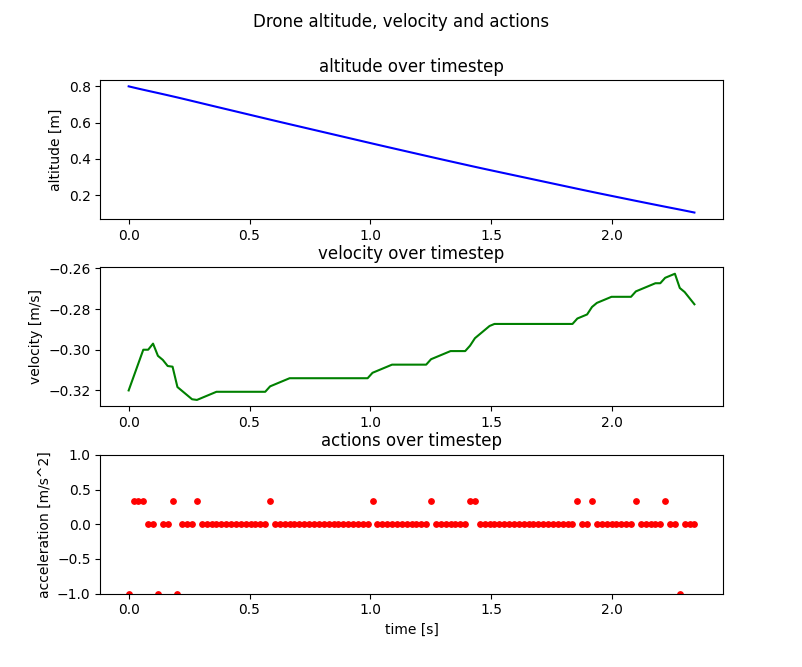
\includegraphics[width=.45\textwidth]{Figures/drone_landing_seed50_drone_snn_pos_06-05-02.png}
    \caption{Performance of an SNN based controller on the basic simulation model.}
    \label{fig:basic performance}
\end{figure}

To analyze whether the network exploits the velocity information rather than applying a fixed thrust, an experiment was run with a zero initial velocity. Now, the network is initially hesitant in commanding negative acceleration commands, slowing down the landing. When the network achieved approached landing, the network commanded more and more positive acceleration, slowing down the MAV upon landing as seen on \autoref{fig:Performance0vel}.

\begin{figure}[h!]
    \centering
    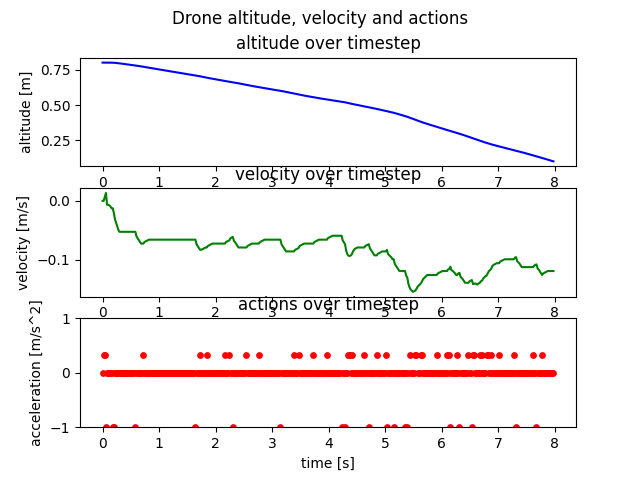
\includegraphics[width=.45\textwidth]{chapters/drone_landing_seed3_v00_drone_snn_pos_06-05-02.png}
    \caption{Performance of an SNN based controller on the basic simulation model, with a zero initial velocity.}
    \label{fig:Performance0vel}
\end{figure}

Next, the same network was deployed in the PaparazziUAV simulator environment. In this setup, the network's acceleration commands were mapped to throttle settings for the Parrot Bebop 2 MAV. To facilitate this, the model was converted into C code, which was then wrapped in a module compatible with PaparazziUAV. This C code is wrapped in a module, which can be used by a PaparazziUAV airframe. The airframe defines the characteristics of the MAV, the sensors that will be used and the controllers that control the MAV. Then, a flight plan is set up, which defines the trajectory to be followed. The flight plan consists of a take-off, a short standby period, and the landing with the SNN based controller.
Due to the coarse discretization of the controller, which outputs only seven distinct commands, the MAV's ability to finely adjust the thrust settings was limited. To address this, the range of thrust settings was constrained between $10\%$ and $70\%$, ensuring that the controller could effectively manage the MAV's thrust within these bounds.

Finally, the network was deployed on the real MAV. It was found that slight instabilities occurred which were not present in simulation. While this could partially be caused by the coarseness of the output actions, but are most likely caused by imperfect tuning of the underlying stabilization controllers, which were provided by the PaparazziUAV framework. On \autoref{fig:real_drone}, the path of the MAV is provided, for the interested reader, a video has been provided as well\footnote{\url{https://youtu.be/16wEXy7pPSM}}.
\begin{figure}
    \centering
    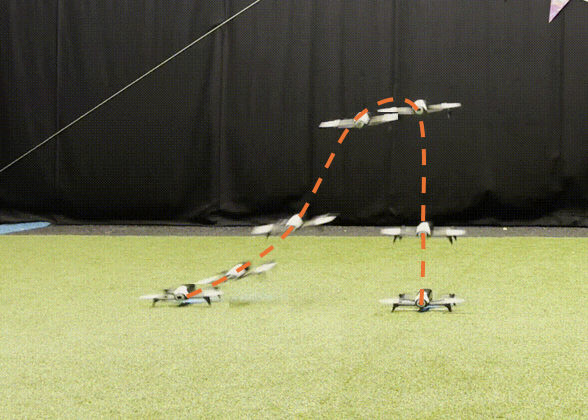
\includegraphics[width=.45\textwidth]{Figures/drone_landing/Drone_Landing_Burst.png}
    \caption{The controller deployed on the real MAV can successfully land}
    \label{fig:real_drone}
\end{figure}

